
\documentclass[tikz,convert={convertexe={magick.exe}}]{standalone}
\usetikzlibrary{snakes}

\begin{document}
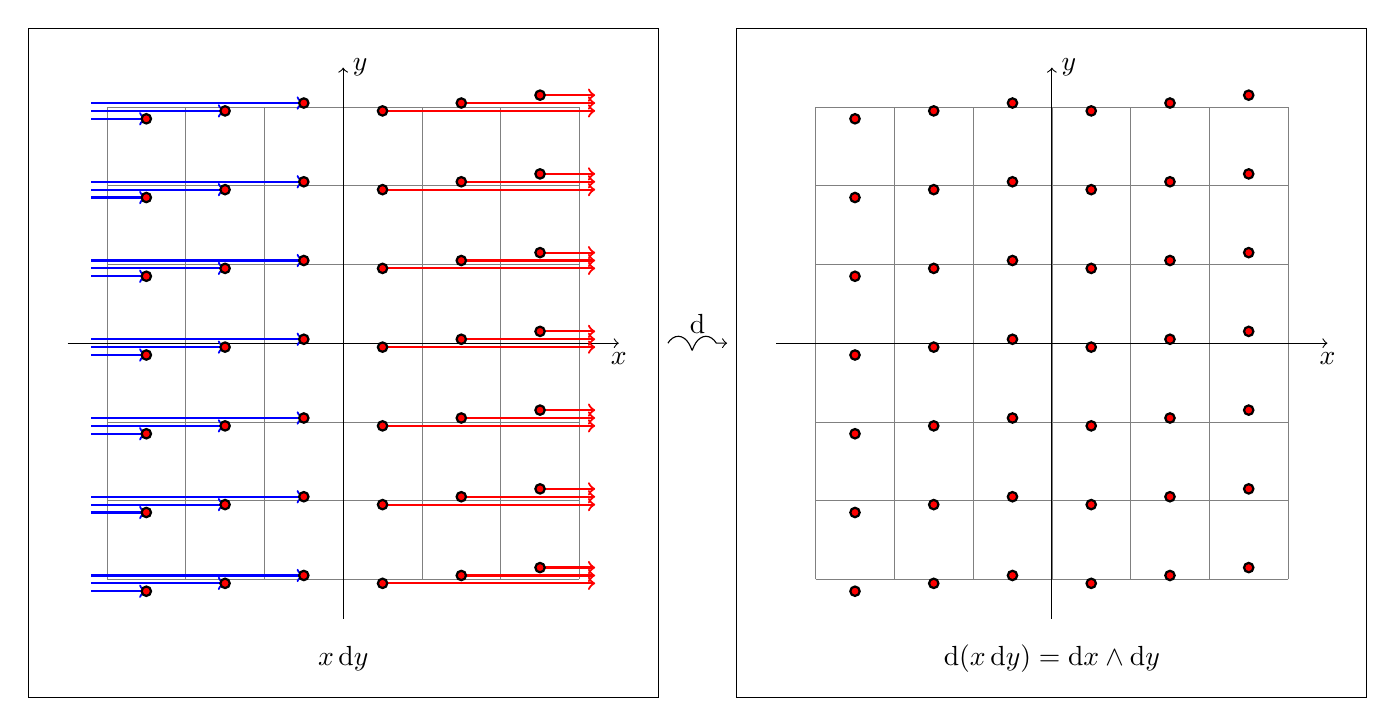
\begin{tikzpicture}

\tikzstyle atom=[circle, draw, inner sep=1.2pt, fill=red, thick]

\begin{scope}

\foreach \x in {-3,-2,...,3}
\draw[style=help lines, very thin] (\x,-3) -- (\x,3);
\foreach \y in {-3,-2,...,3}
\draw[style=help lines, very thin] (-3,\y) -- (3,\y);

\draw[->] (-3.5,0)--(3.5,0) node[below] {$x$};
\draw[->] (0,-3.5)--(0,3.5) node[right] {$y$};

\node (P) at (4,0) {};

\draw (-4,-4.5) rectangle (4,4);
\node at (0,-4) {$x \, \mathrm{d}y$};

\draw[red,->, thick] (0.500,-3.050)--(3.200,-3.050);
\node[atom] at (0.500,-3.050) {};
\draw[blue,->, thick] (-3.200,-2.950)--(-0.500,-2.950);
\node[atom] at (-0.500,-2.950) {};
\draw[red,->, thick] (0.500,-2.050)--(3.200,-2.050);
\node[atom] at (0.500,-2.050) {};
\draw[blue,->, thick] (-3.200,-1.950)--(-0.500,-1.950);
\node[atom] at (-0.500,-1.950) {};
\draw[red,->, thick] (0.500,-1.050)--(3.200,-1.050);
\node[atom] at (0.500,-1.050) {};
\draw[blue,->, thick] (-3.200,-0.950)--(-0.500,-0.950);
\node[atom] at (-0.500,-0.950) {};
\draw[red,->, thick] (0.500,-0.050)--(3.200,-0.050);
\node[atom] at (0.500,-0.050) {};
\draw[blue,->, thick] (-3.200,0.050)--(-0.500,0.050);
\node[atom] at (-0.500,0.050) {};
\draw[red,->, thick] (0.500,0.950)--(3.200,0.950);
\node[atom] at (0.500,0.950) {};
\draw[blue,->, thick] (-3.200,1.050)--(-0.500,1.050);
\node[atom] at (-0.500,1.050) {};
\draw[red,->, thick] (0.500,1.950)--(3.200,1.950);
\node[atom] at (0.500,1.950) {};
\draw[blue,->, thick] (-3.200,2.050)--(-0.500,2.050);
\node[atom] at (-0.500,2.050) {};
\draw[red,->, thick] (0.500,2.950)--(3.200,2.950);
\node[atom] at (0.500,2.950) {};
\draw[blue,->, thick] (-3.200,3.050)--(-0.500,3.050);
\node[atom] at (-0.500,3.050) {};
\draw[red,->, thick] (1.500,-2.950)--(3.200,-2.950);
\node[atom] at (1.500,-2.950) {};
\draw[blue,->, thick] (-3.200,-3.050)--(-1.500,-3.050);
\node[atom] at (-1.500,-3.050) {};
\draw[red,->, thick] (1.500,-1.950)--(3.200,-1.950);
\node[atom] at (1.500,-1.950) {};
\draw[blue,->, thick] (-3.200,-2.050)--(-1.500,-2.050);
\node[atom] at (-1.500,-2.050) {};
\draw[red,->, thick] (1.500,-0.950)--(3.200,-0.950);
\node[atom] at (1.500,-0.950) {};
\draw[blue,->, thick] (-3.200,-1.050)--(-1.500,-1.050);
\node[atom] at (-1.500,-1.050) {};
\draw[red,->, thick] (1.500,0.050)--(3.200,0.050);
\node[atom] at (1.500,0.050) {};
\draw[blue,->, thick] (-3.200,-0.050)--(-1.500,-0.050);
\node[atom] at (-1.500,-0.050) {};
\draw[red,->, thick] (1.500,1.050)--(3.200,1.050);
\node[atom] at (1.500,1.050) {};
\draw[blue,->, thick] (-3.200,0.950)--(-1.500,0.950);
\node[atom] at (-1.500,0.950) {};
\draw[red,->, thick] (1.500,2.050)--(3.200,2.050);
\node[atom] at (1.500,2.050) {};
\draw[blue,->, thick] (-3.200,1.950)--(-1.500,1.950);
\node[atom] at (-1.500,1.950) {};
\draw[red,->, thick] (1.500,3.050)--(3.200,3.050);
\node[atom] at (1.500,3.050) {};
\draw[blue,->, thick] (-3.200,2.950)--(-1.500,2.950);
\node[atom] at (-1.500,2.950) {};
\draw[red,->, thick] (2.500,-2.850)--(3.200,-2.850);
\node[atom] at (2.500,-2.850) {};
\draw[blue,->, thick] (-3.200,-3.150)--(-2.500,-3.150);
\node[atom] at (-2.500,-3.150) {};
\draw[red,->, thick] (2.500,-1.850)--(3.200,-1.850);
\node[atom] at (2.500,-1.850) {};
\draw[blue,->, thick] (-3.200,-2.150)--(-2.500,-2.150);
\node[atom] at (-2.500,-2.150) {};
\draw[red,->, thick] (2.500,-0.850)--(3.200,-0.850);
\node[atom] at (2.500,-0.850) {};
\draw[blue,->, thick] (-3.200,-1.150)--(-2.500,-1.150);
\node[atom] at (-2.500,-1.150) {};
\draw[red,->, thick] (2.500,0.150)--(3.200,0.150);
\node[atom] at (2.500,0.150) {};
\draw[blue,->, thick] (-3.200,-0.150)--(-2.500,-0.150);
\node[atom] at (-2.500,-0.150) {};
\draw[red,->, thick] (2.500,1.150)--(3.200,1.150);
\node[atom] at (2.500,1.150) {};
\draw[blue,->, thick] (-3.200,0.850)--(-2.500,0.850);
\node[atom] at (-2.500,0.850) {};
\draw[red,->, thick] (2.500,2.150)--(3.200,2.150);
\node[atom] at (2.500,2.150) {};
\draw[blue,->, thick] (-3.200,1.850)--(-2.500,1.850);
\node[atom] at (-2.500,1.850) {};
\draw[red,->, thick] (2.500,3.150)--(3.200,3.150);
\node[atom] at (2.500,3.150) {};
\draw[blue,->, thick] (-3.200,2.850)--(-2.500,2.850);
\node[atom] at (-2.500,2.850) {};

\end{scope}

\begin{scope}[xshift=9cm]

\foreach \x in {-3,-2,...,3}
\draw[style=help lines, very thin] (\x,-3) -- (\x,3);
\foreach \y in {-3,-2,...,3}
\draw[style=help lines, very thin] (-3,\y) -- (3,\y);

\draw[->] (-3.5,0)--(3.5,0) node[below] {$x$};
\draw[->] (0,-3.5)--(0,3.5) node[right] {$y$};

\node (Q) at (-4,0) {};

\draw (-4,-4.5) rectangle (4,4);
\node at (0,-4) {$\mathrm{d}(x \, \mathrm{d}y) = \mathrm{d} x \wedge \mathrm{d} y$};

\node[atom] at (0.500,-3.050) {};
\node[atom] at (-0.500,-2.950) {};
\node[atom] at (0.500,-2.050) {};
\node[atom] at (-0.500,-1.950) {};
\node[atom] at (0.500,-1.050) {};
\node[atom] at (-0.500,-0.950) {};
\node[atom] at (0.500,-0.050) {};
\node[atom] at (-0.500,0.050) {};
\node[atom] at (0.500,0.950) {};
\node[atom] at (-0.500,1.050) {};
\node[atom] at (0.500,1.950) {};
\node[atom] at (-0.500,2.050) {};
\node[atom] at (0.500,2.950) {};
\node[atom] at (-0.500,3.050) {};
\node[atom] at (1.500,-2.950) {};
\node[atom] at (-1.500,-3.050) {};
\node[atom] at (1.500,-1.950) {};
\node[atom] at (-1.500,-2.050) {};
\node[atom] at (1.500,-0.950) {};
\node[atom] at (-1.500,-1.050) {};
\node[atom] at (1.500,0.050) {};
\node[atom] at (-1.500,-0.050) {};
\node[atom] at (1.500,1.050) {};
\node[atom] at (-1.500,0.950) {};
\node[atom] at (1.500,2.050) {};
\node[atom] at (-1.500,1.950) {};
\node[atom] at (1.500,3.050) {};
\node[atom] at (-1.500,2.950) {};
\node[atom] at (2.500,-2.850) {};
\node[atom] at (-2.500,-3.150) {};
\node[atom] at (2.500,-1.850) {};
\node[atom] at (-2.500,-2.150) {};
\node[atom] at (2.500,-0.850) {};
\node[atom] at (-2.500,-1.150) {};
\node[atom] at (2.500,0.150) {};
\node[atom] at (-2.500,-0.150) {};
\node[atom] at (2.500,1.150) {};
\node[atom] at (-2.500,0.850) {};
\node[atom] at (2.500,2.150) {};
\node[atom] at (-2.500,1.850) {};
\node[atom] at (2.500,3.150) {};
\node[atom] at (-2.500,2.850) {};

\end{scope}


\draw[snake=coil, ->] (P) -- (Q) node[midway, above] {$\mathrm{d}$};

\end{tikzpicture}
\end{document}